What we call an entity is an object or set of objects in the world that are mentioned in the text. An entity mention could be a name, a noun phrase or a pronoun that refers to a certain entity. \cite{LDC2016.rich_ere} Entities can be any kind of thing, but we choose to only annotate persons, organizations, companies, countries and places.

\begin{exe}
    \ex \annxpl{\anntrg{Schotland} voert \anntrg{minimumprijs} voor \anntrg{alcohol} in.}
        \expl \annxpl{Schotland,} \annxpl{minimumprijs} and \annxpl{alcohol} are all entity mentions that denote entities -- but only \annxpl{Schotland} is interesting for us.
    \ex \annxpl{\anntrg{De Schotse premier} maakt zich sterk dat \anntrg{heel wat landen in Europa en daarbuiten} het voorbeeld zullen volgen van \anntrg{Schotland}.}
        \expl Entity mentions can span many words and denote entire groups of entities.
    \ex \annxpl{\anntrg{Ze} merkte op dat bijvoorbeeld \anntrg{Ierland} en \anntrg{Wales} gelijkaardige plannen hebben.}
        \expl Pronouns can be entity mentions too. When many entities are mentioned in a list, it's usually better to think of them as many separate entities rather than as one group of entities.
\end{exe}

It's important to remember that \textbf{we only annotate entities that are arguments to an event.} We annotate events first, then look for the entities that the event asks for as arguments. If an entity does not have a role as an event argument, we do not annotate it.

For every entity mention, we annotate: 
\begin{el}
    § The mention extent: the maximal continuous string of text that indicates the entity.
    § The entity type: person (PER), organization (ORG), geopolitical entity (GPE), location (LOC) or facility (FAC).
    § The mention level type (NAM, NOM or PRO):
        §§ Named: the entity is referred to by its name (\annxpl{\anntrg{Theresa May} gave a speech\ldots)}
        §§ Nominal: a common noun or noun phrase (\annxpl{\anntrg{The prime minister of the UK} gave a speech\ldots})
        §§ Pronominal: a pronoun (\annxpl{\anntrg{She} gave a speech\ldots})
    § If the mention level type is nominal, we also annotate the head of the mention, ie. the single principal word in the construction (\annxpl{The \annhead{chairman} of the board,} \annxpl{a rather handsome \annhead{man}})
    § Specificity:
        §§ Specific: the referent is a real thing you can point to in the real world.
        §§ Non-specific: generic (\annxpl{\anntrg{lawyers} don’t work for free}) or underspecified (\annxpl{\anntrg{many people} will attend}).
        §§ Remark: when in doubt, ask yourself: can I point my finger at the entity in real life? If a group, are the boundaries of the group well-defined? If so, it's probably specific. "Eight people died in the blast" has a specific group of entities; "many have died" is underspecified (not a well-defined group).
    § If specific, we also annotate individuality: individual, group or unknown.
\end{el}

See figure \ref{fig:rich_ere_ann_categories} for a summary of this system.

\begin{figure}[t]
\centering
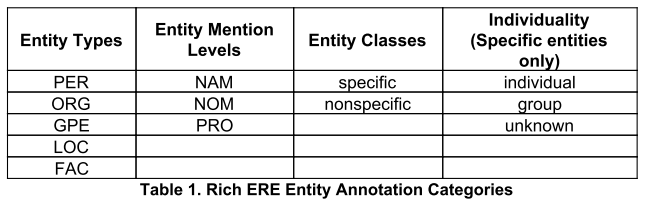
\includegraphics[width=\textwidth]{img/rich_ere_ann_categories.png}
\caption{Summary table of Rich ERE entity annotation, from \cite{LDC2016.rich_ere}.}
\label{fig:rich_ere_ann_categories}
\end{figure}


\section{Entity types}

This section is reproduced from \cite{LDC2016.rich_ere}. We label five entity types in Rich ERE. There are no entity subtypes.

\begin{el}
    § Person (PER) - Person entities are limited to humans. A PER entity may be a single person or a group.
    § Organization (ORG) - Organization entities are corporations, agencies, and other groups of people defined by an established organizational structure. An ORG entity may be a single organization or a group. NOTE: A key feature of an ORG is that it can change members without changing identity.
    § Geopolitical Entity (GPE) - GPE entities are composite entities, consisting of a physical location, a government, and a population. All three of these elements must be present for an entity to be tagged as a GPE. A GPE entity may be a single geopolitical entity or a group.
    § Location (LOC) - Location entities are geographical entities such as geographical areas and landmasses, bodies of water, and geological formations. A LOC entity may be a single location or a group.
    § Facility (FAC) – A facility is a functional, primarily man-made structure. Facilities are artifacts falling under the domains of architecture and civil engineering.
\end{el}



\section{NAM, NOM and PRO}

\textbf{Named entities} (NAM) are represented by a proper name, \textbf{nominal entities} (NOM) by a nominal phrase, and \textbf{pronominal entities} (PRO) by some sort of pronoun. For nominal entities, you additionally annotate a \textbf{head}, which is the single word (rarely a group of words) that represents the entity most succinctly. It is usually the syntactic head of the noun phrase. In these examples, the marked portion is the entire entity mention and the bold part is the head.

\begin{exe}
    \ex \annxpl{\anntrg{Een jonge \annhead{vrouw} uit het West-Vlaamse Staden} kwam om het leven.} 
    \expl \type{PER, NOM, Spec, Indiv}
    
    \ex \annxpl{Onder \anntrg{de \annhead{slachtoffers}} zijn ook \anntrg{vier \annhead{Belgen.}}} 
    \expl \annxpl{De slachtoffers:} \type{PER, NOM, Spec, Group.} \annxpl{Vier Belgen}: \type{PER, NOM, Spec, Group.}
    
    \ex \annxpl{\anntrg{Twaalf \annhead{anderen}} raakten gewond.}
    \expl \type{PER, NOM, Spec, Group.} In a phrase like \annxpl{twaalf anderen}, it seems difficult to find the head. Syntactically, however, \annxpl{twaalf} modifies \annxpl{anderen}, which is therefore the head.
\end{exe}

When a name is given as part of a nominal construction, you only annotate the name as a Named entity. The rest of the construction is not relevant; the name takes precedence. 

\begin{exe}
    \ex \annxpl{Eerste minister \anntrg{Malcolm Turnbull} leidt sinds 2005 de Liberale Partij.}
    
    \ex \annxpl{De Russische dubbelspion \anntrg{Sergej Skripal} en \anntrg{zijn dochter}.}
\end{exe}

Names of countries used as an adjective are not annotated as entities.

\begin{exe}
    \ex \annxpl{\anntrg{De Russische dubbelspion} werd gisteren vergiftigd.}
    \expl \annxpl{De Russische dubbelspion} is an entity, \annxpl{Russische} is not.
\end{exe}

We annotate entities in a fine-grained way: when you find a group of entities in which the consituents are identified separately, annotate each as a separate entity.

\begin{exe}
    \ex \annxpl{Uit protest tegen de vergiftiging van de Russische ex-dubbelspion \anntrg{Sergej Skripal} in het Britse \anntrg{Salisbury} gaan \anntrg{Europa}, de \anntrg{VS} en \anntrg{Canada} \anntrg{Russische \annhead{diplomaten}} uitwijzen.}
        \expl \annxpl{Sergej Skripal} \type{PER, NOM, Spec, Indiv}
        \expl \annxpl{Salisbury} \type{LOC, NOM, Spec, Indiv}
        \expl \annxpl{Europa} \type{LOC, NOM, Spec, Indiv}
        \expl \annxpl{VS} \type{LOC, NOM, Spec, Indiv}
        \expl \annxpl{Canada} \type{LOC, NOM, Spec, Indiv}
        \expl \annxpl{Russische diplomaten} \type{LOC, NOM, Spec, Group}
\end{exe}

Entities expressed by a \textbf{pronoun} must also be tagged. Pronouns can be anaphoric, in which case they refer to some previous entity in the sentence, or they may stand alone. Remember that we annotate on the sentence level: if a pronoun has an antecedent, it occurs in the same sentence. For us, however, the distinction does not matter: we annotate all pronouns as separate entities, regardless of their anaphoric character. This means that if a pronoun occurs in a sentence alongside its antecedent, and both are the argument of an event, both must be annotated as such. The identity between them is established by co-reference links in another stage of the annotation process.

\begin{exe}
    % stand-alone pronoun example.
    \ex \annxpl{President \anntrg{Trump} noemt \anntrg{Saipov} een beest en dreigt ermee \anntrg{hem} naar \anntrg{Guantanamo} te sturen.} 
    \expl \annxpl{Sturen} triggers a \type{Movement.\-Transport\-Person} event with \annxpl{Trump} as agent and \annxpl{Guantanamo} as destination. The person being transported is expressed twice: \annxpl{Saipov} and \annxpl{hem}. The event is annotated with two separate Person arguments.
    % anaphoric pronoun example.
    
\end{exe}






